\textbf{Работа 3.2.5}

\textbf{Вынужденные колебания в электрическом контуре.}

Цель работы: исследование вынужденных колебаний и процессов их
установления в колебательном контуре.

\emph{В работе используются: генератор звуковых частот, осциллограф,
вольтметр, частотомер, конденсатор, катушка индуктивности, магазин
сопротивлений, универсальный мост.}

\emph{В работе исследуются колебания, возникающие в параллельном
электрическом контуре под действием внешнего гармонического генератора
тока. }

При подключении к контуру внешнего источника в нём возникают колебания,
которые можно представить как суперпозицию двух синусоид (2.72): первая
с частотой собственных колебаний контура и амплитудой, экспоненциально
убывающей со временем; вторая с частотой внешнего источника и постоянной
амплитудой. Со временем собственные колебания затухают, и в контуре
устанавливаются вынужденные колебания. Амплитуда этих колебаний
максимальна при резонансе совпадении частоты внешнего сигнала с
собственной частотой контура 0. Зависимость амплитуды установившихся
колебаний от частоты внешнего напряжения носит название
«\emph{резонансная кривая».}

\textbf{А. Резонансная кривая колебательного контура.}

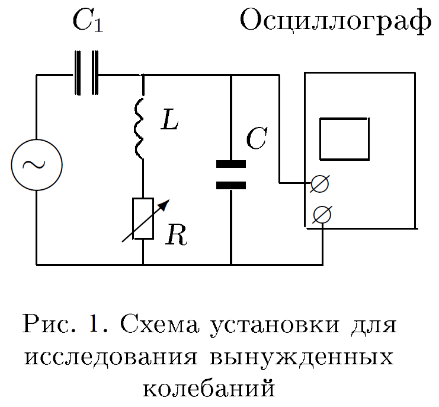
\includegraphics[width=1.99792in,height=1.85in]{./media/image1.png}Для
экспериментального исследования резонансной кривой напряжения в
параллельном колебательном контуре используется схема, изображенная на
рисунке 1. Синусоидальный сигнал с генератора подаётся на параллельный
колебательный контур через небольшую разделительную ёмкость C1.
Напряжение с конденсатора контура C поступает на вертикальный вход
электронного осциллографа (ЭО). Для снятия резонансной кривой
необходимо, чтобы импедансы возбуждающей и измеряющей цепей
(сопротивления переменному току) намного превосходили импеданс самого
контура вблизи резонанса Zрез ≈ L/(RC) = Q/(ΩC). Разделительная ёмкость
C1 выбирается настолько малой, что в рабочем диапазоне частот её
импеданс ZC1 = 1/(ΩC1) много больше импеданса контура, поэтому в цепи
генератора течёт ток практически с постоянной амплитудой, а
колебательный контур выполняет роль нагрузочного сопротивления, которое,
в свою очередь, зависит от частоты. Поскольку в резонансе сопротивление
Zрез параллельного контура максимально, то и напряжение на ёмкости C
(неизменный ток, умноженный на максимальное сопротивление) тоже
максимально. Входное сопротивление осциллографа (измеряющей цепи)
достаточно велико: Rэо ≈ 1 МОм, поэтому его влиянием можно пренебречь.

Таким образом, при выполнении условий

\[Z_{C_{1}} = \frac{1}{\mathrm{\Omega}C_{1}} \gg \left| Z \right|_{rez} = \frac{Q}{\text{ΩC}}\ ,\ \ \ \ \ \ \ R_{EO} \gg \frac{Q}{\text{ΩC}}\ \ \ \ \ \ \ \ \ \ \ \ \ \ \ \ \ (1)\]

и при условии, что действительная часть импеданса катушки много меньше
её мнимой части, резонансная кривая в нашем контуре будет выглядеть так
же, как и в последовательном: максимум амплитуды при резонансе. Ширина
резонансной кривой определяет важную характеристику контура --
\emph{добротность}.

\textbf{Б. Процессы установления и затухания колебаний в контуре.}

Добротность контура может быть определена и другими способами, например,
по скорости нарастания амплитуды вынужденных колебаний при резонансе или
по скорости затухания свободных колебаний.

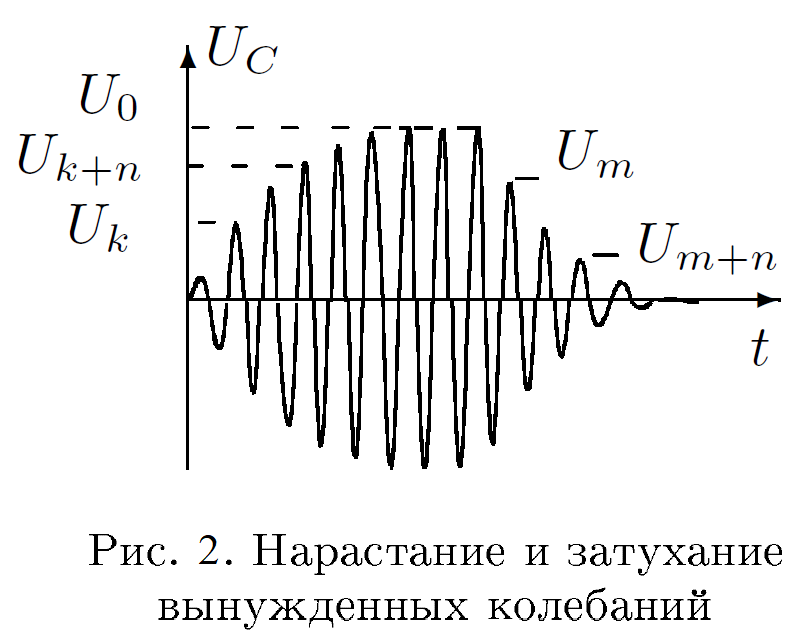
\includegraphics[width=2.72431in,height=2.17778in]{./media/image2.PNG}Нарастание
и затухание колебаний (рис. 2) можно наблюдать на экране осциллографа,
если на контур подаются цуги - отрезки синусоиды, разделённые
интервалами, в течение которых сигнал отсутствует. Чем выше добротность,
тем медленнее нарастают и медленнее затухают колебания в контуре.
Количественные оценки можно сделать, если определить логарифмический
декремент затухания по скорости нарастания или затухания колебаний. В
условиях резонанса огибающая затухающих колебаний - это перевёрнутая
огибающая нарастающего участка, поэтому при расчёте логарифмического
декремента по затуханию нет необходимости использовать амплитуду
установившихся колебаний U0, которая в контуре с высокой добротностью
может не успеть установиться за время продолжительности цуга.

\textbf{Экспериментальная установка.} Схема установки для исследования
вынужденных колебаний приведена на рис. 3. Колебательный контур состоит
из конденсатора с ёмкостью C, катушки с индуктивностью L и магазина
сопротивлений R.

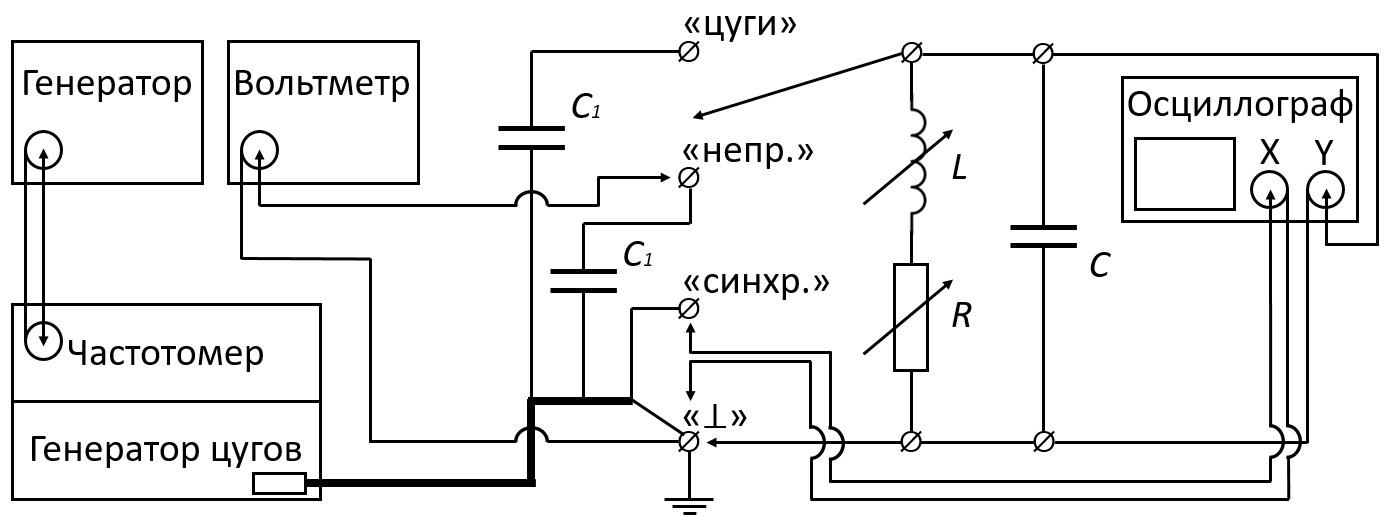
\includegraphics[width=6.49653in,height=2.48056in]{./media/image3.png}

Рис. 3. Схема экспериментальной установки для исследования вынужденных
колебаний.

Синусоидальное напряжение от звукового генератора проходит через
частотомер, позволяющий измерять рабочую частоту с высокой точностью, и
генератор цугов -- электронное реле, ``разрезающее'' синусоиду на
периодически повторяющиеся цуги -- отрезки синусоиды.

Затем сигнал через небольшую ёмкость C1 поступает на клеммы,
смонтированные на отдельной панели. При подключении контура к клеммам
«⊥» и «непр.» на контур подаётся непрерывный сигнал -- синусоида; если
контур подключён к клеммам «⊥» и «цуги» - на контур поступают отрезки
синусоиды.

Для наблюдения за процессом колебаний напряжение с ёмкости подаётся на
вход осциллографа. Чтобы картина на экране была устойчивой, частота
развёртки осциллографа принудительно синхронизуется с частотой
повторения цугов. Для этого на генератор развёртки ЭО подаются следующие
с частотой повторения цугов управляющие импульсы, которые вырабатываются
в блоке электронного реле (клемма «синхр», смонтированная на панельке).
Для измерений напряжения на ёмкости используется электронный вольтметр.

\textbf{ЗАДАНИЕ}

В работе предлагается при двух значениях сопротивления магазина
исследовать резонансные кривые и определить по ним добротность контура;
затем определить добротность, определив логарифмический декремент
затухания при нарастании и при затухании колебаний.

I. Подготовка приборов к работе

1. Соберите схему согласно рис. 4 и подключите контур к клеммам «⊥» и
«непр.». Включите приборы в сеть. Руководствуясь техническим описанием,
расположенным у установки, настройте генератор, осциллограф, проверьте
работоспособность источника питания, а также выставите необходимые
значения на магазинах сопротивлений и индуктивностей.

II. Исследование резонансных кривых

2. Рассчитайте собственную частоту контура
\(\nu_{0} = 1/2\pi\sqrt{\text{LC}}\).

3. Изменяя частоту генератора вблизи резонансной и наблюдая за
синусоидой на экране осциллографа, убедитесь, что в резонансе амплитуда
колебаний максимальна. Подберите частоту развёртки осциллографа и
амплитуду синхронизации, при которых картина неподвижна.

4. Меняя частоту генератора в обе стороны от резонансной, снимите
зависимость показаний вольтметра \emph{U} от показаний частотомера
\emph{ν}. Расчёт добротности ведётся на уровне 0,7 от резонансной
амплитуды, поэтому стоит аккуратнее провести измерения в районе этого
уровня, а также продолжать измерения по крайней мере до тех пор, пока
амплитуда сигнала упадёт до величины 0,3--0,4 от резонансной.

5. Установите на магазине сопротивлений другое значение, заданное
преподавателем, и повторите измерения п.4. Закончив измерения, отключите
вольтметр от сети.

III. Процессы установления и затухания колебаний.

6. Подключите контур к клеммам «цуги» и «⊥». Выведите до нуля
сопротивление магазина.

7. Установите на генераторе резонансную частоту. Подберите частоту
развёртки осциллографа, при которой на экране умещается один цуг
колебаний. Убедитесь, что огибающая затухающих колебаний это
перевёрнутая огибающая нарастающего участка. Если они заметно отличаются
(реле может внести искажения), то следует уменьшить амплитуду сигнала с
генератора.

8. Для расчёта добротности по скорости нарастания амплитуды измерьте
амплитуды двух колебаний Uk и Uk+n, разделённых целым числом периодов n,
и амплитуду установившихся колебаний U0 (см. рис. 2).

Перед началом измерений заземлите канал Y, чтобы уточнить положение оси
X -- начала отсчёта амплитуды. Можно увеличить амплитуду, сместив
горизонтальную ось симметрии цуга в нижнюю часть экрана. Расчёт будет
тем точнее, чем больше отличаются друг от друга все три амплитуды.

Проведите измерения для 3--4-х пар амплитуд.

9. Для определения добротности по скорости затухания измерьте две
амплитуды, разделённые целым числом периодов (для 3--4-х пар амплитуд).

10. Повторите измерения п.8 и п.9 для другого значения сопротивления,
заданного преподавателем.

11. Сместите частоту генератора от резонансного значения и получите на
экране картину биений. Зарисуйте и объясните эту картину.

12. Отключите приборы от сети и разберите схему.

13. Измерьте активное сопротивление RL и индуктивность L магазина
индуктивностей с помощью измерителя LCR на частотах 50 Гц, 500 Гц и 1500
Гц.

IV. Обработка результатов

1. Постройте на одном графике резонансные кривые в координатах U/U0 = f(
ν/ν0), где U0 -- напряжение при резонансной частоте ν0.

Определите добротность по формуле Q = ω0/(2ΔΩ). Сравните теоретическое и
экспериментальное значения резонансной частоты.

2. Рассчитайте добротность контура по скорости нарастания и затухания
колебаний.

3. Рассчитайте теоретическое значение добротности через параметры
контура L, C и R.

4. Сведите результаты определения Q в таблицу:

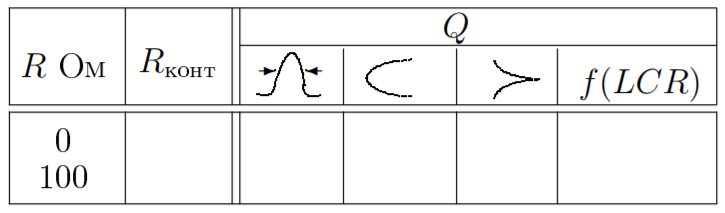
\includegraphics[width=3.37592in,height=0.99167in]{./media/image4.png}

5. Оцените погрешности и сравните результаты расчётов.

\emph{Список литературы.}

1. Сивухин Д.В. Общий курс физики. -- Т.III. Электричество. -- М.:
Физматлит, 2004. §§ 122 -- 124.

2. Калашников С.Г. Электричество. -- М.: Физматлит, 2008. §§ 207 -- 210.
